\chapter{Návrh a architektura aplikace}

\section{Serverová část}

Rozdělení do projektů:

TODO: u každé dopodrobna rozepsat co obsahuje, k čemu slouží + ukázky kódu

\subsection{Data}

Tento projekt se stará primárně o komunikaci s databází, pro tento účel jsme použili ORM framework Entity Framework Core. 

Ve složce Models jsou třídy reprezentující databázové entity. Každá z entit pak v databázi představuje jednu tabulku. V aplikaci jsme použili tyto entity:

\begin{table}[ht]
	\centering
	\resizebox{\textwidth}{!}{
	\begin{tabular}{| l | l |}
		Entita & reprezentuje \\
		a & členství uživatele v daném kurzu. K této entitě se pak vážou všechny známky a odeslané testy.
	\end{tabular}
}
\end{table}

\begin{itemize}
	\item Course -- tato entita reprezentuje kurz
	\item CourseFile - reprezentuje nějaký soubor sdílený v kurzu
	\item CourseMember - představuje členství uživatele v daném kurzu. K této entitě se pak vážou všechny známky a odeslané testy.
	\item CourseTest - představuje jeden test v kurzu
	\item ForumPost - slouží k reprezentaci příspěvků ve fóru k danému kurzu
	\item Grade - reprezentuje známku kterou student obdržel (kromě známek z testů)
	\item Person - reprezentuje uživatele aplikace
	\item TestQuestion - reprezentuje 1 otázku v testu
	\item TestSubmission - reprezentuje test s odpověďmi odeslaný uživatelem
	\item TestSubmissionAnswer - představuje odpověď k dané otázce v testu
\end{itemize}

\newpage

\begin{figure}
	\centering
	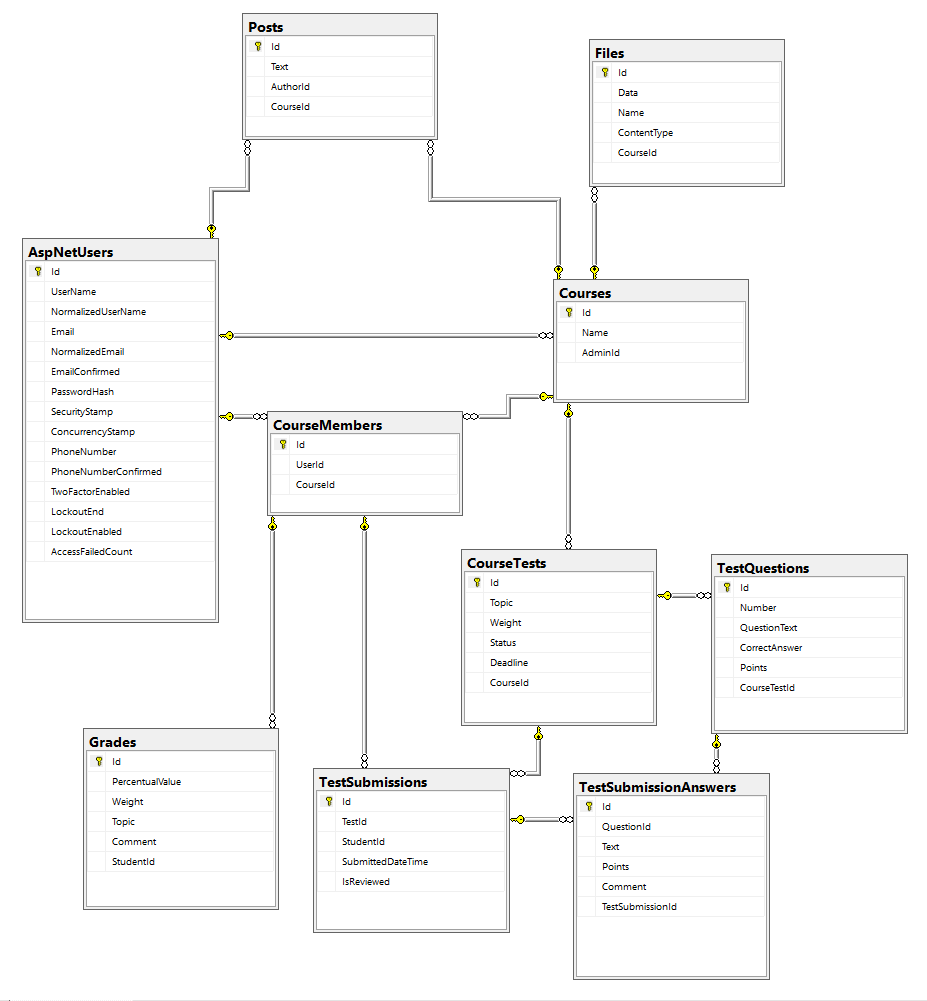
\includegraphics[width=\textwidth]{db_model.PNG}
	\caption{Databázový model aplikace}
\end{figure}

\newpage

např. kód třídy Course vypadá takto:

\begin{lstlisting}
public class Course : IGuidIdObject
{
	public Course()
	{
		Members = new List<CourseMember>();
		Files = new List<CourseFile>();
		Tests = new List<CourseTest>();
		ForumPosts = new List<ForumPost>();
	}
	
	public Course(string name, Person admin) : this()
	{
		Name = name;
		Admin = admin;
	}
	
	/// <summary>
	/// identifier of the couse
	/// </summary>
	[DatabaseGenerated(DatabaseGeneratedOption.Identity)]
	[Key]
	public Guid Id { get; set; }
	
	/// <summary>
	/// name of the course
	/// </summary>
	[Required]
	public string Name { get; set; }
	
	...
\end{lstlisting}

Vidíme, že každá entita obsahuje veřejné vlastnosti (public properties) s gettery a settery. Tyto vlastnosti budou v databázové tabulce reprezentovány jako sloupce. Některé z nich (jako např. Id) obsahují ještě doplňující atributy, ty slouží k upřesnění informací o dané vlastnosti. Například atribut [Key] určuje, že tato vlastnost bude v databázi primární klíč, atribut [Required] určuje, že daný sloupec bude v tabulce u všech záznamů povinný (tedy hodnoty budou NOT NULL).
Dále musí každá entita obsahovat konstruktor bez parametrů.

Vazby mezi entitami jsou reprezentované pomocí tzv. navigačních vlastností. V případě, že chceme vytvořit vazbu typu one-to-many mezi entitami A a B, stačí do vlastností třídy A přidat kolekci objektů typu B, a naopak do třídy B vlastnost typu A. Framework pak při provádění migrace vytvoří v databázové tabulce entity B vytvoří sloupec s cizím klíčem, který bude obsahovat identifikátor entity A, ke které patří.

V aplikaci je vazba one-to-many použita mimo jiné mezi entitami Course a CourseTest, a to tak, že každý test je obsažen v právě jednom kurzu, a v daném kurzu může být N testů.
Kód pak tedy vypadá takto: ve třídě Course je kolekce objektů typu CourseTest

\begin{lstlisting}
/// <summary>
/// tests in this course
/// </summary>
public ICollection<CourseTest> Tests { get; set; }
\end{lstlisting}

a ve třídě CourseTest je pak vlastnost typu Course

\begin{lstlisting}
/// <summary>
/// course that contains this test
/// </summary>
[Required]
public Course Course { get; set; }
\end{lstlisting}

Po provedení databázové migrace (viz. dále) se v tabulce CourseTest vytvoří sloupec CourseId s cizím klíčem, který odkazuje na identifikátor kurzu (tzn. vlastnost Course.Id).

Také si můžeme všimnout, že všechny entity (kromě entity Person) implementují rozhraní IGuidObject. To je jednoduché rozhraní, které obsahuje pouze jednu vlastnost - Id typu Guid. Tímto máme zajištěnou jednotu identifikátorů, tedy že všechny entity, které toto rozhraní implementují, budou mít identifikátor typu Guid.

\begin{lstlisting}
/// <summary>
/// interface for object with <see cref="Guid"/> identifier
/// </summary>
public interface IGuidIdObject
{
	/// <summary>
	/// identifier of the object
	/// </summary>
	Guid Id { get; set; }
}
\end{lstlisting}


Typ Guid jsme zvolili hlavně z toho důvodu, že vestavěné tabulky frameworku (např. Identity) mají také řetězcové identifikátory. Navíc se pak zjednoduší práce ve frontend části (není potřeba parsovat string na int např. v klientské části při práci s URL). Tyto identifikátory generuje databáze, takže je zajištěno, že jsou unikátní.
Další možnost by byla použít jako identifikátor číslo (např. typ int), ale vzhledem k výše uvedeným argumentům je typ Guid v tomto případě lepší možnost.

Dále se v projektu nachází také rozhraní ICourseReferenceObject a ICourseMemberReferenceObject, které slouží k tomu, abychom mohli dále v aplikaci jednotně pracovat s objekty, které mají referenci na entitu Course, resp. CourseMember. Tyto rozhraní implementují pouze nějaké entity.

V programu je dále třída CMSDbContext, která reprezentuje databázový kontext této aplikace. Každý objekt typu DbSet pak představuje jednu databázovou tabulku. Ve třídě je CMSDbContext tedy kolekce typu DbSet pro každou z entit.

\begin{lstlisting}
public DbSet<Grade> Grades { get; set; }

public DbSet<Course> Courses { get; set; }

...
\end{lstlisting}

Jediná výjimka je entita Person, která dědí ze třídy IdentityUser, a jejíž DbSet je nakonfigurovaný ve frameworku. 

V programu pak dále používáme ke komunikaci s databází pouze třídu CMSDbContext a objekty typu DbSet. Třida DbSet<TEntity> implementuje rozhraní IQueryable<TEntity>, takže na ní lze použít LINQ. Takže pokud bych chtěl například vybrat všechny kurzy, jejiž jméno začíná na písmeno C, pak stačí použít následující LINQ dotaz
\begin{lstlisting}
dbContext.Courses.Where(course => course.Name.StartsWith("C"))
\end{lstlisting}
kde proměnná dbContext je instance třídy CMSDbContext.

Ve třídě CMSDbContext je také metoda ConfigureForeignKeys, která provede konfiguraci cizích klíčů v aplikaci. Všechny políčka s cizími klíči jsou v databázi povinné (tzn. NOT NULL), to je zajištěno pomocí atributu [Required] daných vlastností. Nastavením DeleteBehavior.Restrict u cizích klíčů zajistíme, že databáze zůstane v konzistentním stavu. Pokud bychom tedy chtěli smazat entitu, pak na ní nesmí pomocí cizích klíčů odkazovat jiné entity. V opačném případě program při zavolání metody SaveChanges() na databázovém kontextu vyhodí výjimku.

V programu je dále složka Migrations. Při vývoji byl použit princip Code first, tedy že v kódu specifikujeme entity pomocí klasických tříd. Framework se pak postará o vytvoření databázových tabulek z tohoto kódu.

Pokud jsem tedy nějak změníme některou z entit (to může být např. přidání vlastnosti, změna jména vlastnosti, apod.), pak pomocí ORM můžeme vygenerovat soubor popisující tzv. databázovou migraci, která slouží k aplikaci změn z kódu do databáze. Ke každé migraci se vygeneruje jeden soubor, který obsahuje popis změn, které se později provedou v databázi.

K vytváření migrací jsem použijeme nástroj CLI tools for Entity Framework Core. https://docs.microsoft.com/cs-cz/ef/core/cli/dotnet. Pro vygenerování migrace ze změn v kódu použijeme příkaz:

\begin{lstlisting}
dotnet ef migrations add {migration_name} 
--project CourseManagementSystem.Data 
--startup-project CourseManagementSystem.API
\end{lstlisting}

Tímto se vytvoří soubor popisující změny v migraci, ale databáze zatím zůstala beze změny. Tento soubor obsahuje třídu, jenž dědí ze třídy Migration a obsahuje metody Up a Down. V metodě Up je popis změn, které se provedou při aplikaci této migrace, naopak v metodě Down je popis změn, které se provedou v případě odstranění migrace.

Jako příklad si můžeme představit migraci, která obsahuje přidání vlastnosti ScoreWeight k entitě CourseTest (tato vlastnost popisuje váhu testu).
Vygenerovaný kód migrace vypadá takto:

\begin{lstlisting}
public partial class TestWeight_added : Migration
{
	protected override void Up(MigrationBuilder migrationBuilder)
	{
		migrationBuilder.AddColumn<int>(
		name: "ScoreWeight",
		table: "CourseTests",
		nullable: false,
		defaultValue: 0);
	}
	
	protected override void Down(MigrationBuilder migrationBuilder)
	{
		migrationBuilder.DropColumn(
		name: "ScoreWeight",
		table: "CourseTests");
	}
}
\end{lstlisting}

Pro promítnutí změn do databáze následně použijeme příkaz:

\begin{lstlisting}
dotnet ef database update 
--project CourseManagementSystem.Data 
--startup-project CourseManagementSystem.API
\end{lstlisting}

Tímto tedy dojde k změnám v databázi (v našem příkladu se vytvoří sloupec ScoreWeight v tabulce CourseTests).

V obou příkazech je potřeba specifikovat cílový a startup projekt. Cílový projekt je ten, který obsahuje databázový kontext a entity naší aplikace (v tomto případě projekt Data). Naopak startup projekt je projekt, který je spouštěný frameworkem, což je potřeba pro získání konfiguračních informací o projektu, jako je například connection string do naší databáze.

\newpage

\subsection{Services}
V tomto projektu se nachází pomocné služby pro komunikaci s databází. 

Jako základ pro všechny služby slouží abstraktní třída DbService, která obsahuje referenci na databázový kontext aplikace a jedinou metodu CommitChanges(). Ta slouží k uložení změn provedených v databázovém kontextu do databáze. 

To je potřeba, protože k uložení změn do databáze dojde až tehdy, když na databázovém kontextu zavoláme metodu SaveChanges(). Pokud bychom tedy například do databázového kontextu něco uložili (např. takto: 
\begin{lstlisting}
dbContext.Grades.Add(new Grade())
\end{lstlisting}
a nezavolali metodu dbContext.SaveChanges(), data by se neuložila.

\begin{lstlisting}
/// <summary>
/// class representing base database service
/// </summary>
public abstract class DbService : IDbService
{
	/// <summary>
	/// context of the CMS database
	/// </summary>
	protected readonly CMSDbContext dbContext;
	
	/// <summary>
	/// construct a new database service
	/// </summary>
	/// <param name="dbContext">CMS database context</param>
	protected DbService(CMSDbContext dbContext)
	{
		this.dbContext = dbContext;
	}
	
	/// <inheritdoc/>
	public void CommitChanges()
	{
		dbContext.SaveChanges();
	}
}
\end{lstlisting}

Tato třída implementuje rozhraní IDbService, které obsahuje pouze metodu CommitChanges().

Dále jsou ve složce Interfaces rozhraní pro další služby, ty jsou rozdělené podle entit (typicky máme pro jednu entitu jednu službu). Všechny tyto rozhraní také implementují rozhraní IDbService. 

Například rozhraní ICourseService (slouží pro práci s kurzy) vypadá takto:
\begin{lstlisting}
public interface ICourseService : IDbService
{
	/// <summary>
	/// get course by its id
	/// </summary>
	/// <param name="courseId">identifier of the course</param>
	/// <returns></returns>
	Course GetById(string courseId);
	
	/// <summary>
	/// archive course by its id
	/// </summary>
	/// <param name="courseId">id of the course to delete</param>
	void ArchiveById(string courseId);
	
	/// <summary>
	/// add the course into the database
	/// </summary>
	/// <param name="course">course to add</param>
	void AddCourse(Course course);
	...
\end{lstlisting}

Ve složce Implementations jsou potom implementace těchto rozhraní. Můžeme vidět, že všechny implementace dědí ze třídy DbService, a zároveň také tranzitivně implementují IDbService.

Například třída CourseService, která implementuje rozhraní ICourseService vypadá takto:

\begin{lstlisting}
public class CourseService : DbService, ICourseService
{
	public CourseService(CMSDbContext dbContext) : base(dbContext)
	{ }
	
	/// <inheritdoc/>
	public void ArchiveById(string courseId)
	{
		Course c = GetById(courseId);
		c.IsArchived = true;
	}
	
	/// <inheritdoc/>
	public Course GetById(string courseId)
	{
		return dbContext.Courses.FindById(courseId);
	}
	
	/// <inheritdoc/>
	public void AddCourse(Course course)
	{
		dbContext.Courses.Add(course);
	}
	...
\end{lstlisting}

Vidíme, že služby typicky pracují s databázovým kontextem, a s daty (vyhledávání, mazání, apod.).
Dále si můžeme všimnout, že v žádné metodě se neukládájí změny do databáze (tzn. volání metody CommitChanges()). To je z toho důvodu, že ve vyšších vrstvách aplikace (např. API) v jedné metodě často voláme několik služeb, příp. několik metod z jedné služby. 
Pokud bychom v metodách služeb přímo ukládali změny do databáze (metoda CommitChanges()), pak bychom se mohli lehce dostat to nekonzistentního stavu. To například tak, že při volání několika služeb v rámci jedné metody by 
mohla některá ze služeb vyhodit výjimku, nicméně všechny služby zavolané předtím by už data uložily.

Takže je na zodpovědnosti volajícího provést uložení změn do databáze, tedy zavolat metodu CommitChanges(), což je typicky poslední příkaz v dané metodě.
Tím jsme tedy zajistili konzistenci dat - buď se do databáze uloží všechny změny provedené v databázovém kontextu, nebo žádné.

Dále si můžeme všimnout, že ve službách pracujeme s identifikátory typu string, ale v databázi používáme typ Guid. To je z toho důvodu, že ve vyšších vrstvách aplikace se pohodlněji pracuje se stringy (např. často dostáváme ID jako URL parametr). Převod mezi typy string a Guid pak řešíme ve službách.

Ve složce Extensions jsou pak pomocné extension metody pro práci s některými třídami.

Ve třídě DbSetExtensions se nachází extension metody pro třídu DbSet<T>. Vybereme si například metodu GetCourseIdOf, ta slouží k získání ID kurzu, ke kterému daný objekt, jenž má referenci na entitu Course, patří.
\begin{lstlisting}
/// <summary>
/// get id of <see cref="Data.Models.Course"/> that the object belongs to
/// </summary>
/// <typeparam name="T">type of items</typeparam>
/// <param name="dbSet">database set</param>
/// <param name="objectId">identifier of the object we look for in <paramref name="dbSet"/></param>
/// <returns></returns>
public static string GetCourseIdOf<T>(this DbSet<T> dbSet, string objectId) where T : class, ICourseReferenceObject, IGuidIdObject
{
	return dbSet.Include(item => item.Course)
		.Single(item => item.Id.ToString() == objectId)
		.Course.Id.ToString();
}
\end{lstlisting}

Vidíme, že toto je jeden z příkladů použití rozhraní ICourseReferenceObject, které se nachází v projektu Data.

V projektu též máme rozhraní ICourseReferenceService, to implementují všechny služby, jejichž entity logicky patří k nějakému kurzu. Rozhraní obsahuje jedinou metodu GetCourseIdOf(string objectId), která získá ID kurzu, ke kterému daná entita patří. V implementaci této metodu pak typicky používáme extension metodu GetCourseIdOf pro třídu DbSet<T>. Například ve třídě CourseTestService vypadá implementace takto:

\begin{lstlisting}
public string GetCourseIdOf(string objectId)
{
	return dbContext.CourseTests.GetCourseIdOf(objectId);
}
\end{lstlisting}

Podobně je v projektu i rozhraní ICourseMemberReferenceService, které používají služby, jejichž entity mají referenci na třídu CourseMember.

Použitím služeb jsme odstranili duplikátní kód (např. hledání kurzu podle ID se používá na několika místech ve vyšších vrstvách), a extrahovali některé složitější dotazy do samostatných metod. To je výhodné hlavně z toho důvodu, že je pak můžeme nezávisle otestovat. Další výhoda je, že vyšší vrstvy jsou odstíněny od použití ORM (a databázového kontextu), pouze volají tyto služby.

+ eager loading

\newpage

\subsection{API}

obsahuje Controllery, ViewModels, komunikace s klientskou částí

\subsection{Tests}

obsahuje testy služeb

\section{Klientská část}

\subsection{Components}

slouží k zobrazování dat, každá komponenta má 2 části: šablonu a backend

\subsection{Services}

slouží ke komunikaci klienta se server části

\subsection{ViewModels}

reprezentují objekty, které se používají v komunikaci s API

\section{Zajímavé problémy}

\subsection{Použití Dependency injection}

TODO: popsat použití + ukázat příklad

\subsection{ViewModels x DB entity}

Použil jsem různé objekty pro databázové entity a view-modely.

TODO: pořádně rozepsat + vysvětlit + ukázka kódu

\subsection{ViewModels v serverové i klientské části}

view-modely jsou v serverové i klientské části aplikace

TODO: pořádně rozepsat + vysvětlit + ukázka kódu

\subsection{Uživatelské role}

V systému je několik rolí, serverová část provádí autorizaci.

TODO: pořádně rozepsat typy rolí + autorizaci
